\documentclass[10pt]{beamer}

%%%
% PREAMBLE FOR THIS DOC 
%%%
%https://tex.stackexchange.com/questions/68821/is-it-possible-to-create-a-latex-preamble-header
\usepackage{/Users/miw267/Repos/latex_preamble/beamer_preamble}

\usetikzlibrary{matrix}


%%% WARNING SIGN
\usepackage{fontawesome5}



%%%
% DOCUMENT
%%%

\begin{document}

%\maketitle

%% Title page frame
%\begin{frame}
%    \titlepage 
%\end{frame}




\title{11/2/2026: Intro to Probability (Part 1)}
\author{CSCI 246: Discrete Structures}
\date{Textbook reference: Sec 30, Scheinerman}

\begin{frame}
    \titlepage 
\end{frame}


\begin{frame}
\footnotesize 
\begin{mygreenbox}[title=Graded Quiz Pickup]
Quizzes are in the front of the room, grouped into four bins (A-G, H-L, M-R, S-Z) by last name. The quizzes are upside down with your last name on the back. Come find yours before, during, or after class.  Only turn the quiz over if it's yours.
\end{mygreenbox} 
\vfill 

%\begin{myredbox}[title=Announcements]
%\begin{itemize}
%	\item Please sign the attendance sheet.
%\end{itemize}
%\end{myredbox}

\vfill 


\begin{myyellowbox}[title=Today's Agenda]
\begin{itemize}
	\item Follow up from last class ($\approx$ 10 mins)
	\item Mini-lecture ($\approx$ 25 mins)
	\item Group exercises ($\approx$ 15 mins)
\end{itemize}
\end{myyellowbox}
\vfill 


\begin{myredbox}[title=Follow-up from last class]
\begin{enumerate}
\item Fixed for loops to be Python (with exclusive for loops)   
\item Why Big O is not worst case.
\item Why we like Big O/Big Theta.
\end{enumerate}
\end{myredbox}


 
\end{frame}

\begin{frame}[standout]
Feedback on Weekly Quiz \#8
\end{frame}


\begin{frame}{Recall: Weekly Quiz \#7}
\footnotesize 
\begin{figure}[ht]
        \centering
        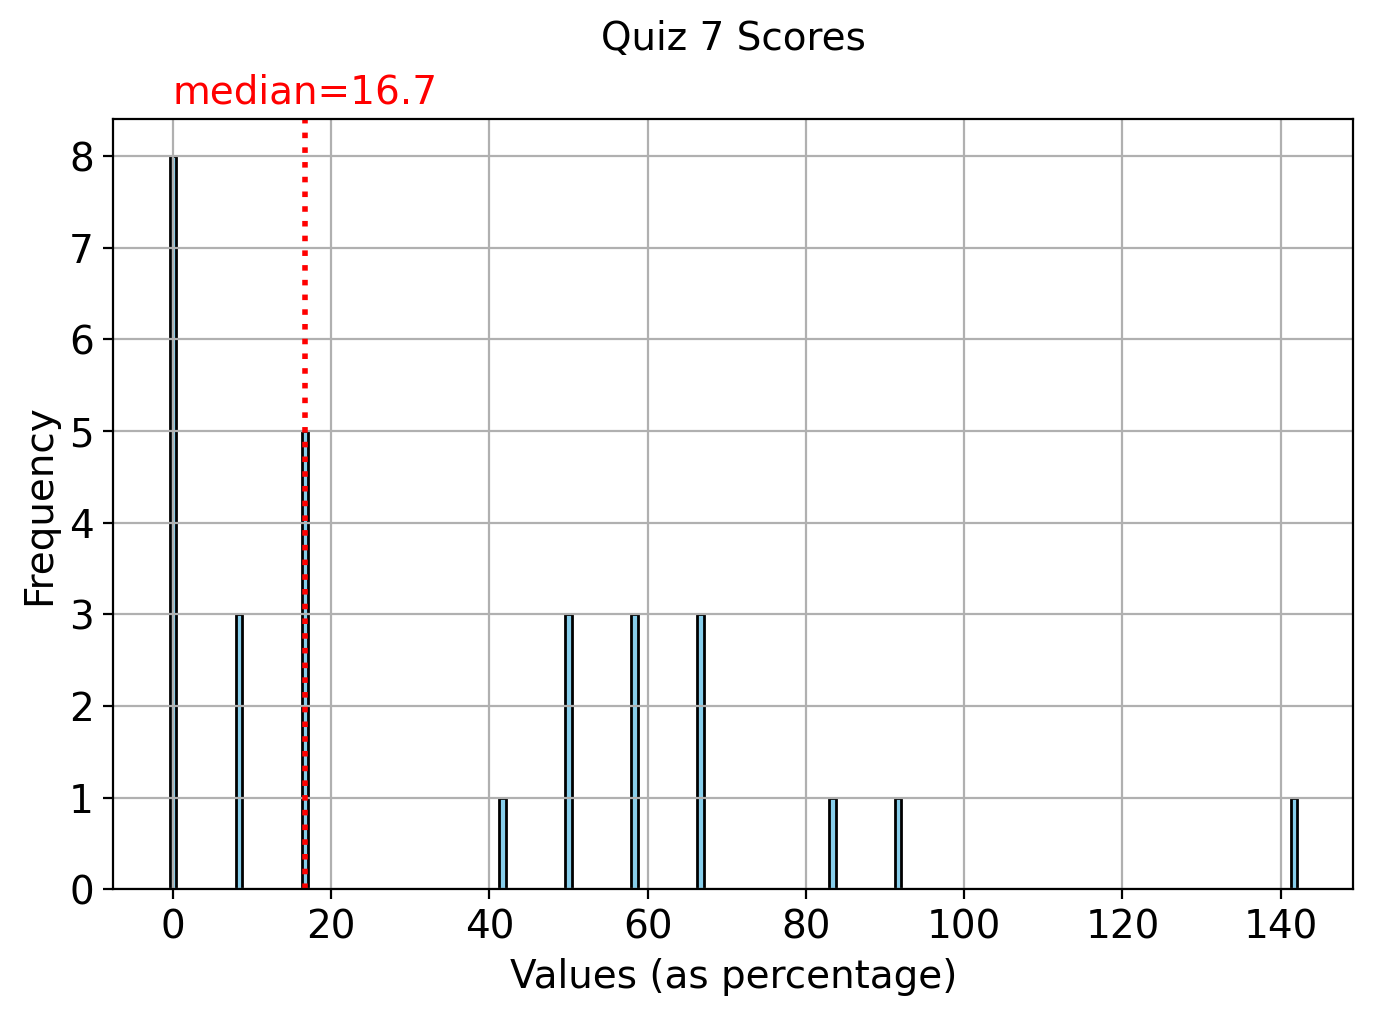
\includegraphics[width=.8\textwidth]{images/quiz_7_histogram}
\end{figure}
\vfill 
\end{frame}	

\begin{frame}{Weekly Quiz \#8}
\footnotesize 
\begin{figure}[ht]
        \centering
        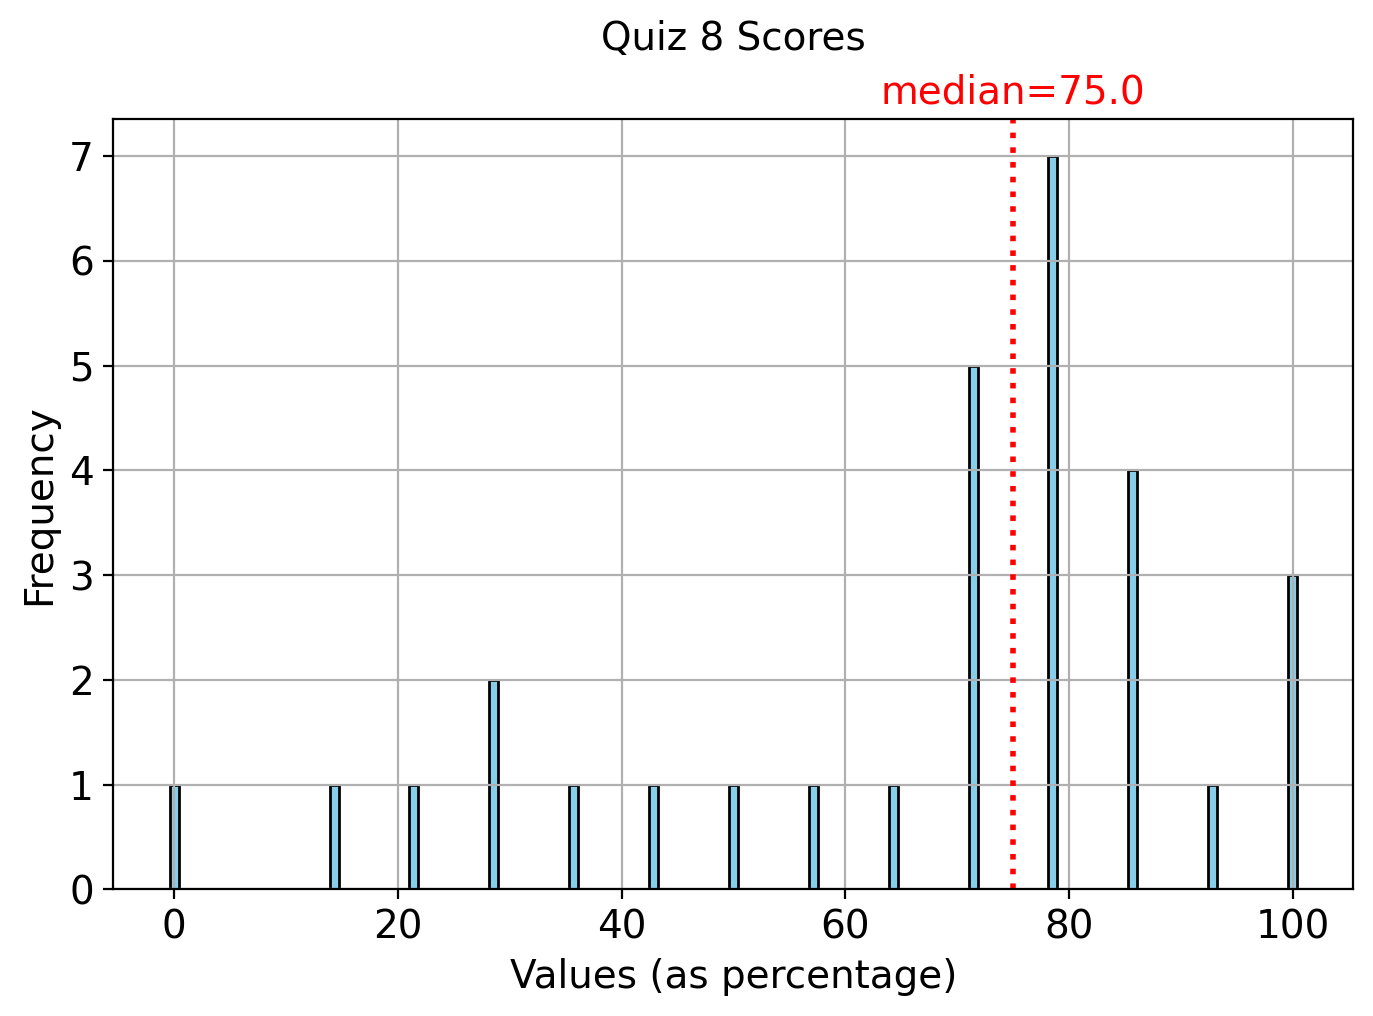
\includegraphics[width=.8\textwidth]{images/quiz_8_histogram}
\end{figure}
\vfill 
\end{frame}	






\begin{frame}[standout]
Introduction to Probability: \\
Samples and Events
\end{frame}


%
\begin{frame}{Example: Drawing a card from a well-shuffled deck}



\centering
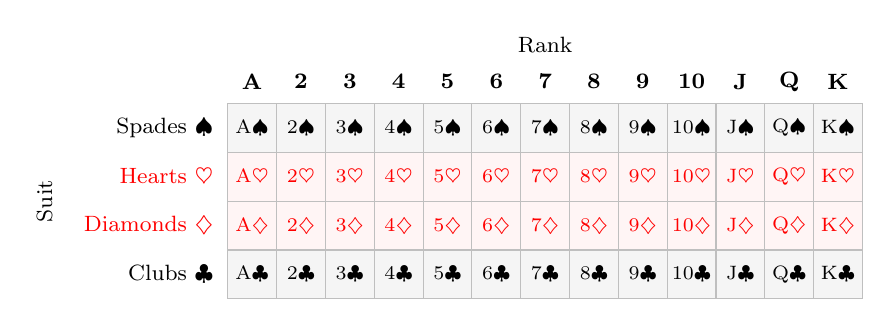
\begin{tikzpicture}[x=0.62cm, y=0.62cm, every node/.style={font=\scriptsize}]
  \def\ranks{{"A","2","3","4","5","6","7","8","9","10","J","Q","K"}}
  % suit symbol, color
  \foreach \s/\sym/\col [count=\r from 0] in
      {Spades/\spadesuit/black, Hearts/\heartsuit/red, Diamonds/\diamondsuit/red, Clubs/\clubsuit/black} {
    % row label
    \node[anchor=east, text=\col, font=\footnotesize] at (-0.1, -\r - 0.5) {\s\ $\sym$};
    \foreach \c in {0,...,12} {
      \pgfmathsetmacro{\rk}{\ranks[\c]}
      \draw[gray!50, fill=\col!4] (\c, -\r) rectangle (\c+1, -\r-1);
      \node[text=\col] at (\c+0.5, -\r-0.5) {\rk$\sym$};
    }
  }
  % column labels
  \foreach \c in {0,...,12} {
    \pgfmathsetmacro{\rk}{\ranks[\c]}
    \node[font=\footnotesize\bfseries] at (\c+0.5, 0.45) {\rk};
  }
  % axis titles
  \node[font=\footnotesize, anchor=south] at (6.5, 0.85) {Rank};
  \node[font=\footnotesize, rotate=90, anchor=south] at (-3.4, -2) {Suit};
\end{tikzpicture}
%
\vfill 
\raggedright
\only<2->{\colorbox{blue!30}{\textbf{Remark.}} A standard deck: 4 suits $\times$ 13 ranks = 52 cards}

\vfill \vfill 
\only<3->{Consider drawing a card from a well-shuffled deck.}
\only<4->{The outcome is \alert{random.}}

\vfill 
\only<5->{What is the space of possible outcomes (the \textbf{sample space})?} \only<6->{\alert{The 52 cards shown above.}}  \only<7->{\alert{We can write 	$S= \set{A \spadesuit, A \heartsuit, A \diamondsuit, A \clubsuit, 2 \spadesuit, \hdots, K \clubsuit}$. }}
\vfill
\only<8->{What is the probability of each outcome?} \only<9->{\alert{Since each outcome is equally likely, each outcome has the same probability: $\frac{1}{52}.$}}
\vfill
\end{frame}
%
%\begin{frame}
%
%\begin{myyellowbox}[title=Poll]
%Imaging tossing two coins and observing whether 0, 1, 2 heads are obtained.  Will each of these events occur about 1/3 of the time?
%\end{myyellowbox}
%
%\pause 
%\vfill 
%
%\begin{figure}
%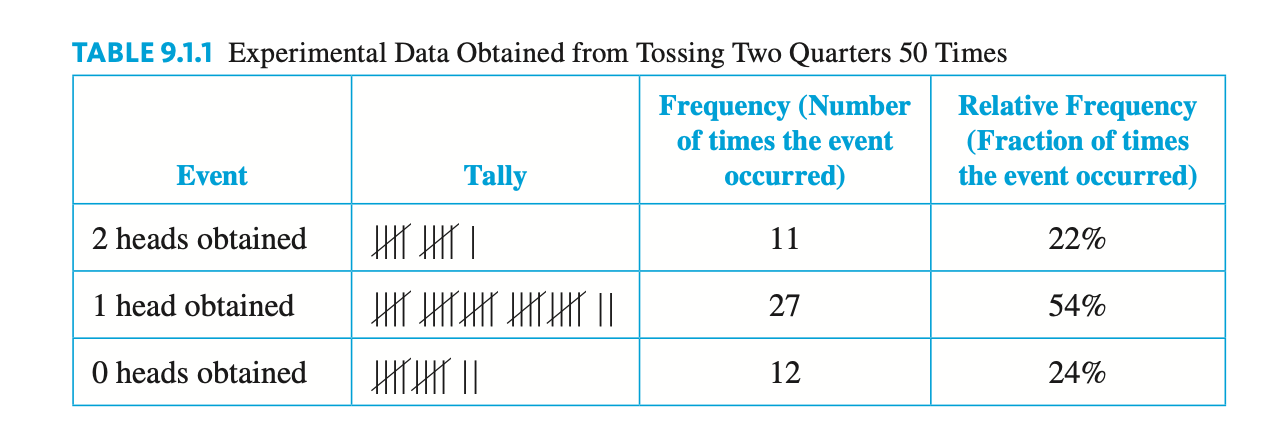
\includegraphics[width=.8\textwidth]{images/coins_1.png}	
%\end{figure}
%
%Empirically, 1 head is obtained about twice as often as the other options. Why?  \pause  We'll clarify this matter in the next two slides.
%
%
%
%%\begin{figure}
%%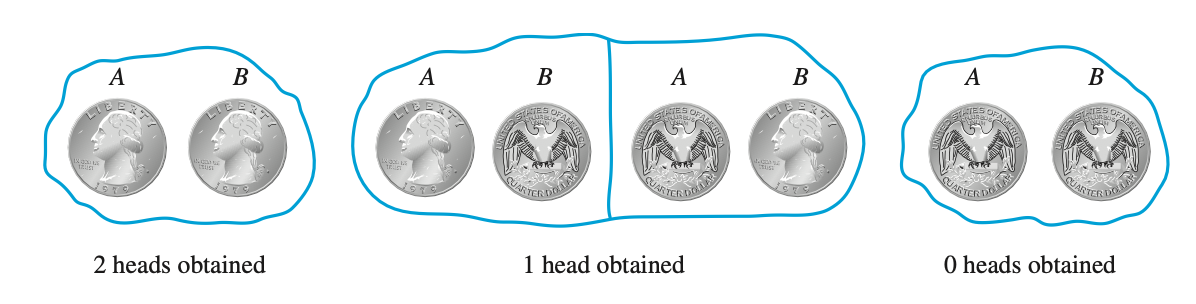
\includegraphics[width=.8\textwidth]{images/coins_2.png}	
%%\end{figure}
%	
%\end{frame}



\begin{frame}{Finite probability spaces}
\small 
\begin{mygreenbox}[title=Definition]
A (finite) \textbf{probability space} is a pair $(S,P)$ where $S$ is a finite, nonempty set and $P$ is a function $S \to \R$ such that $P(s) \geq 0$ for all $s \in S$ and 
\[ \sum_{s \in S} P(s) =1 \] 
\end{mygreenbox}
\vfill 
\pause 
\vfill \vfill 
\colorbox{yellow!30}{\textbf{Poll.}} Do these conditions hold for the example of drawing a playing card? \pause 
\alert{Is $S$ a finite non-empty set?} \pause \greencheck  \pause \alert{Is $P$ a function from $S$ to $\mathbb{R}$ which is non-negative and sums to one?} \pause \greencheck 
\pause 
\vfill \vfill 

\begin{myredbox}[title=\text{Remark: What is a sample space?}]

We refer to $S$ as the \textbf{sample space}: the set of all possible outcomes of a random process or experiment. \\
\pause 
\vfill 
\faExclamationTriangle\ Scheinerman refers to $(S,P)$ as a \textit{sample space}.  However, most people  use \textit{sample space} to refer to $S$ alone.  (We will follow the latter convention.)
\end{myredbox}


%\pause 
%\vfill 
%
%\begin{myyellowbox}[title=Example Of A Probability Space]
%
%In the coin example, we can construct the probability space as 
%\[S = \set{\texttt{HH}, \texttt{HT}, \texttt{TH}, \texttt{TT}} \]
%and $P(s) = 1/4$ for all $s \in S$.
%\end{myyellowbox}

\end{frame}



\begin{frame}{Example: Playing cards}

\begin{mygreenbox}[title=Definition]
An \textbf{event} is a subset of a sample space.  
\end{mygreenbox}


\centering
\begin{tikzpicture}[x=0.62cm, y=0.62cm, every node/.style={font=\scriptsize}]
  \def\ranks{{"A","2","3","4","5","6","7","8","9","10","J","Q","K"}}
  % suit symbol, color
  \foreach \s/\sym/\col [count=\r from 0] in
      {Spades/\spadesuit/black, Hearts/\heartsuit/red, Diamonds/\diamondsuit/red, Clubs/\clubsuit/black} {
    % row label
    \node[anchor=east, text=\col, font=\footnotesize] at (-0.1, -\r - 0.5) {\s\ $\sym$};
    \foreach \c in {0,...,12} {
      \pgfmathsetmacro{\rk}{\ranks[\c]}
      \draw[gray!50, fill=\col!4] (\c, -\r) rectangle (\c+1, -\r-1);
      \node[text=\col] at (\c+0.5, -\r-0.5) {\rk$\sym$};
    }
  }
  % column labels
  \foreach \c in {0,...,12} {
    \pgfmathsetmacro{\rk}{\ranks[\c]}
    \node[font=\footnotesize\bfseries] at (\c+0.5, 0.45) {\rk};
  }
  % axis titles
  \node[font=\footnotesize, anchor=south] at (6.5, 0.85) {Rank};
  \node[font=\footnotesize, rotate=90, anchor=south] at (-3.4, -2) {Suit};
  
  % highlight events
  \only<3>{\draw[orange!90!black, very thick, rounded corners=2pt] (6,0.9) rectangle (7,-4);}
    \only<4>{\draw[orange!90!black, very thick, rounded corners=2pt] (7,0.9) rectangle (8,-4);}
      \only<5-7>{\draw[orange!90!black, very thick, rounded corners=2pt] (6,0.9) rectangle (8,-4);}
      \only<8>{\draw[orange!90!black, very thick, rounded corners=2pt] (0,-1) rectangle (13,-2);}
       \only<9>{\draw[orange!90!black, very thick, rounded corners=2pt] (0,-3) rectangle (13,-3);}
       \only<10-12>{\draw[orange!90!black, very thick, rounded corners=2pt] (0,-1) rectangle (13,-3);}
\end{tikzpicture}
%

\raggedright

\only<2->{
\colorbox{yellow!30}{\textbf{Poll.}} What is an example event when drawing a card from a well-shuffled deck?
} 
\vfill
\only<3->{
\colorbox{red!30}{\textbf{Example.}}}
\only<3>{The event of drawing a 7 is given by 	$E_7= \set{7 \spadesuit, 7 \heartsuit, 7 \diamondsuit, 7 \clubsuit}$.}
\only<4>{The event of drawing a 8 is given by 	$E_8= \set{8 \spadesuit, 8 \heartsuit, 8 \diamondsuit, 8 \clubsuit}$.}
\only<5-7>{The event of drawing a 7 or 8 is given by 	$E_{\text{7 or 8}}= \set{7 \spadesuit, 7 \heartsuit, 7 \diamondsuit, 7 \clubsuit, 8 \spadesuit, 8 \heartsuit, 8 \diamondsuit, 8 \clubsuit}$. } \only<6-7>{\alert{Is there a more compact way to write this?}}\only<7>{\alert{You could write this as $E_{\text{7 or 8}}=E_7 \cup E_8$.}}
\only<8>{The event of drawing a heart is given by 	$E_\heartsuit= \set{A \heartsuit,  2 \heartsuit, \hdots, K \heartsuit}$.}
\only<9>{The event of drawing a diamond is given by 	$E_\diamondsuit= \set{A \diamondsuit,  2 \diamondsuit, \hdots, K \diamondsuit}$.}
\only<10-12>{The event of drawing a red card (a heart or diamond) is given by 	$E_{\text{red}}= \set{A \heartsuit,  2 \heartsuit, \hdots, K \heartsuit, A \diamondsuit,  2 \diamondsuit, \hdots, K \diamondsuit}$. } \only<11-12>{\alert{Is there a more compact way to write this? }} \only<12>{\alert{You could write this as $E_{\text{red}}=E_\heartsuit \cup E_\diamondsuit$.}}
\end{frame}

\begin{frame}{Events and their probabilities}
\begin{mygreenbox}[title=Definition]
Let $(S,P)$ be a probability space.  Then an \textbf{event} $E$ is a subset of $S$ (i.e. $E \subseteq S$).  The probability of an event $E$, denoted $P(E)$ is
%
\begin{align}
P(E) = \sum_{s \in E} P(s) 
\label{eqn:probability_of_event}
\end{align}
\end{mygreenbox}


\vfill 
\only<2->{\colorbox{yellow!30}{\textbf{Poll.}} Describe in words how to construct the probability of an event.}
\vspace{.1cm}
\only<3->{\colorbox{red!30}{\textbf{Solution.}}  Just add up the probabilities of each outcome in the event.}

\vfill 
\only<4-5>{\colorbox{blue!30}{\textbf{Example.}} In the cards example, what is the probability of getting a 7?}
\only<5>{Let $E_7= \set{7 \spadesuit, 7 \heartsuit, 7 \diamondsuit, 7 \clubsuit}$.  Then
\begin{align*}
P(E_7) &= P(7 \spadesuit) + P(7 \heartsuit) + P(7 \diamondsuit) + P(7\clubsuit)  \\
&= \frac{1}{52} + \frac{1}{52} + \frac{1}{52} + \frac{1}{52} \\
& = \frac{4}{52} = \frac{1}{13}. 
\end{align*}
}

\vfill 
\only<6-7>{\colorbox{blue!30}{\textbf{Example.}} In the cards example, what is the probability of getting a 7 or 8?}
\only<7>{Let $E = \set{7 \spadesuit, 7 \heartsuit, 7 \diamondsuit, 7\clubsuit, 8 \spadesuit, 8 \heartsuit, 8 \diamondsuit, 8 \clubsuit}$.   Then
%
\footnotesize 
\begin{align*}
P(E) &= P(7 \spadesuit) + P(7 \heartsuit) + P(7 \diamondsuit) + P(7\clubsuit) +  P(8 \spadesuit) + P(8 \heartsuit) + P(8\diamondsuit) + P(8 \clubsuit) \\
&= \frac{1}{52} + \frac{1}{52} + \frac{1}{52} + \frac{1}{52} +  \frac{1}{52} + \frac{1}{52} + \frac{1}{52} + \frac{1}{52}\\
& = \frac{8}{52} = \frac{2}{13}. 
\end{align*}
}

%
%\only<3>{The event of drawing a 7 is given by 	.}
%\only<4>{The event of drawing a 8 is given by 	$E_8= \set{8 \spadesuit, 8 \heartsuit, 8 \diamondsuit, 8 \clubsuit}$.}
%\only<5-7>{The event of drawing a 7 or 8 is given by 	$E_{\text{7 or 8}}= \set{7 \spadesuit, 7 \heartsuit, 7 \diamondsuit, 7 \clubsuit, 8 \spadesuit, 8 \heartsuit, 8 \diamondsuit, 8 \clubsuit}$. } \only<6-7>{\alert{Is there a more compact way to write this?}}\only<7>{\alert{You could write this as $E_{\text{7 or 8}}=E_7 \cup E_8$.}}
%\only<8>{The event of drawing a heart is given by 	$E_\heartsuit= \set{A \heartsuit,  2 \heartsuit, \hdots, K \heartsuit}$.}
%\only<9>{The event of drawing a diamond is given by 	$E_\diamondsuit= \set{A \diamondsuit,  2 \diamondsuit, \hdots, K \diamondsuit}$.}
%\only<10-12>{The event of drawing a red card (a heart or diamond) is given by 	$E_{\text{red}}= \set{A \heartsuit,  2 \heartsuit, \hdots, K \heartsuit, A \diamondsuit,  2 \diamondsuit, \hdots, K \diamondsuit}$. } \only<11-12>{\alert{Is there a more compact way to write this? }} \only<12>{\alert{You could write this as $E_{\text{red}}=E_\heartsuit \cup E_\diamondsuit$.}}


\end{frame}



\begin{frame}{A shortcut that you can use (\underline{sometimes!})}
\begin{mygreenbox}[title=\text{Proposition: Equally Likely Probability Formula}]
If $(P,S)$ is a probability space in which all outcomes are equally likely and E is an event in $S$, then the probability of $E$ is
%
\begin{align*}
P(E) = \frac{|E|}{|S|} = \frac{\text{the number of outcomes in } E }{\text{the number of outcomes in } S}	
\end{align*}
\end{mygreenbox}

\vfill 
\only<2-3>{\colorbox{blue!30}{\textbf{Example.}} In the cards example, what is the probability of getting a 7 or 8?}
\only<3>{Let $E= \set{7 \spadesuit, 7 \heartsuit, 7 \diamondsuit, 7\clubsuit, 8 \spadesuit, 8 \heartsuit, 8 \diamondsuit, 8 \clubsuit}$.   \alert{Since all outcomes in $E$ are equally likely, we have}
%
\footnotesize
\begin{align*}
P(E) &= \frac{|E|}{|S|} \\
&= \frac{|\set{7 \spadesuit, 7 \heartsuit, 7 \diamondsuit, 7\clubsuit, 8 \spadesuit, 8 \heartsuit, 8 \diamondsuit, 8 \clubsuit}|}{| \texttt{whole deck}|} \\
& = \frac{8}{52} = \frac{2}{13}. 
\end{align*}
}

%\vfill 
%\pause 
%
%\begin{myredbox}[title=Proof]
%\pause 
%\small 
%By the definition of the probability of an event in \Eqref{eqn:probability_of_event}, we have 
%\[ P(E) = \sum_{s \in E} P(s)  \]
%But if all events are equally likely, then $P(s) = c$ for all outcomes $s \in S$.  Hence
%\end{myredbox}

\end{frame}



%
%
%
%\begin{frame}[standout]
%Introduction to Probability: \\
%Some Applications
%\end{frame}
%
%
%\begin{frame}
%\footnotesize 
%\begin{myredbox}[title=Background on cards]
%An ordinary deck of cards contains 52 cards divided into four \textit{suits}.  The \textit{red suits} are 	diamonds ($\diamondsuit$) and hearts ($\heartsuit$), and the \textit{black suits} are clubs ($\clubsuit$) and spades ($\spadesuit$).  Each suit contains 13 cards of the following \textit{denominations}: 2, 3, 4, 5, 6, 7, 8, 9, 10, J (jack), Q (queen), K (king), and A (ace).  The cards J, Q, and K are called \textit{face cards}. 	
%\end{myredbox}
%\vfill 
%\pause 
%\begin{myyellowbox}[title=Poll]
% Suppose we draw a card randomly from a shuffled deck.  (1)  What is the sample space of outcomes? (2) What is the event that the chosen card is a black face card. (3) What is the probability that the chosen card is a black face card?
%\end{myyellowbox}
%\vfill 
%\pause 
%\begin{mygreenbox}[title=Solution]
%\begin{enumerate}
%	\item The sample space $S$ are the 52 cards in the deck.
%	\item \pause 
%	\[E = \set{ J \spadesuit, Q \spadesuit, K \spadesuit, J \clubsuit, Q \clubsuit, K \clubsuit} \] 
%	\item \pause  By the equally likely probability formula,
%	\[ P(E) = \frac{|E|}{|S|} = \frac{6}{52} \approx 11.5\%\]
%\end{enumerate}
%\end{mygreenbox}
%
%
%\end{frame}

\begin{frame}

\begin{myyellowbox}[title=\text{Poll (Practice Reading Quiz)}]
A \textit{hand} of poker is a five-element subset of the standard deck of 52 cards.   Assuming that the deck is well-shuffled, what is the probability of drawing the hand $6 \clubsuit -K \heartsuit - 3 \diamondsuit - A \spadesuit - 7 \clubsuit$?
\end{myyellowbox}
\vfill \vfill 
\pause 

\begin{mygreenbox}[title=\text{Solution}]
Since all poker hands are equally likely, we can use the equally likely probability formula.  Let $S$ be the set of all possible poker hands, and $E$ be the (one-element) set containing the specific poker hand above.  

\vspace{.2cm}

Then
\[P(E) = \frac{|E|}{|S|} = \frac{\text{the number of outcomes in } E }{\text{the number of outcomes in } S}	 = \frac{1}{\binom{52}{5}} = \frac{1}{2,598,960}.\]

\end{mygreenbox}
	
\end{frame}



\begin{frame}
\footnotesize

\begin{myyellowbox}[title=Poll]
\begin{minipage}{.83\textwidth}
A bag contains 20 marbles. These marbles are identical, except that they are labeled with the integers 1 through 20.  Five marbles are drawn randomly from the bag.  What is the probability space?
\end{minipage} %
\hfill 
\begin{minipage}{.15\textwidth}
\begin{figure}
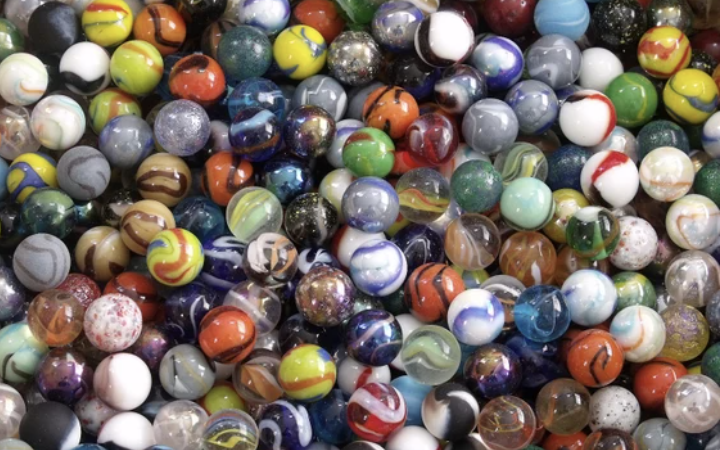
\includegraphics[width=.9\textwidth]{images/marbles}	
\end{figure}
\end{minipage}
\end{myyellowbox}
\vfill 
\begin{myredbox}[title=\text{Solution(s):  \; The solution depends on what's meant by \enquote{randomly}!}]
There are a few ways to think about this.  \pause 
\begin{enumerate} 
	\item \textit{The marbles are drawn one all at once.} Here, we consider the outcomes as sets. Order doesn't matter. So $\set{1,2,3,4,5} = \set{5,4,3,2,1}$. \pause 
	\[ S = \set{\text{subsets of $\set{1,\hdots, 20}$ of size 5}}, |S| = \binom{20}{5}, P(s) = \frac{1}{\binom{20}{5}} \; \forall s \in S \]
	\vspace{-0.3cm}
	\pause \item \textit{The marbles are drawn one at a time without replacement.} Here, we consider the outcomes as lists. Order matters.  $(1,2,3,4,5) \neq (5,4,3,2,1)$. \pause 
	%
	\begin{align*}
	S &= \set{\text{partial permutations of $\set{1,\hdots, 20}$ of size 5}}, \\
	|S| &= (20)_5 = 20 \cdot 19 \cdot 18 \cdot 17 \cdot 16, \quad 
	P(s) = \frac{1}{(20)_5} \; \forall s \in S 	
	\end{align*}
	\vspace{-0.3cm}
	%
\pause \item \textit{The marbles are drawn one at a time with replacement.} Here, we again consider the outcomes as lists, but now $(1,1,1,1,1)$ is possible. \pause  
	\[ S =\set{1,\hdots, 20}^5, |S| = 20^5, P(s) = \frac{1}{20^5} \; \forall s \in S \]
	
\end{enumerate}
\end{myredbox}

\end{frame}





\begin{frame}[standout]
Group exercises
\end{frame}

\begin{frame}{Random group assignments}
%%% TABLE 1: by last name
\begin{columns}
\begin{column}{0.33\textwidth}
Ashley, Isabelle: 2 \\ 
Bailey, Tanna: 6 \\ 
Blaisdell, Olyver: 8 \\ 
Brown, Ashton: 2 \\ 
Cardenas, Dominic: 3 \\ 
Cutler, George: 1 \\ 
Fabik, Roland: 1 \\ 
Fellows, Audrey: 10 \\ 
Fitzgerald, Ryan: 7 \\ 
Fuller, Ryan: 3 \\ 
Griffen, Clara: 2 \\ 
Grutsch, Tanner: 11 \\\end{column}
\begin{column}{0.33\textwidth}
Hager, Nathan: 9 \\ 
Horner, Jayden: 12 \\ 
Johnson, Jaret: 1 \\ 
Kintzel, Samantha: 6 \\ 
Lameres, Alexis: 7 \\ 
Lee, Holden: 11 \\ 
Mayala, Reece: 9 \\ 
McLean, Connor: 6 \\ 
Mcbride, Daniel: 11 \\ 
Miller, Maverick: 5 \\ 
Moss, Emily: 12 \\ 
Mousseau, Matthew: 10 \\\end{column}
\begin{column}{0.33\textwidth}
Neuman, Evan: 12 \\ 
Putnam, John: 5 \\ 
Ramos, Vydel: 3 \\ 
Rathbun, Jedidiah: 7 \\ 
Roberts, Matthew: 10 \\ 
Roller, Nathan: 8 \\ 
Ryan, Otis: 5 \\ 
Shevtsov, Timothy: 4 \\ 
Stensland, Emma: 4 \\ 
Thiessen, Logan: 8 \\ 
Thompson, Jaiden: 4 \\ 
Vath, Ethan: 9 \\\end{column}
\end{columns}
\end{frame}


\begin{frame}{Group exercises}
\small 
\begin{minipage}{.83\textwidth}
\begin{enumerate}
	\item Let $(S,P)$ be the probability space in which $S=\set{1,2,3,4}$. Suppose $P(1) =x, P(2) = 2x, P(3) = 3x,$ and  $P(4)=4x$.  Find $x$.
	\item Suppose that that $(S,P_1)$  and $(S,P_2)$ are two probability spaces that have the same set of outcomes, $S$.   Is it possible that each outcome is less likely in the first probability space than it is in the second?  That is, can we have $\forall s \in S, P_1(s) < P_2(s)$? 
	\item A dart is thrown blindly at the target shown in the figure. The probability that the dart lands in one of the four concentric regions is proportional to the area of the region.  The radii of the circles in the figure are 1,2,3, and 4 units, respectively. Please note that region 2 consists of just the annular region from radius 1 to 2, and does not include the enclosed circular region 1.    Let $(S,P)$ be a probability space modeling this situation.  The set $S$ consists of the four outcomes: hitting region 1,2,3 or 4.  Please find $P(1), P(2), P(3),$ and $P(4)$.  % We can abbreviate that as $S=\set{1,2,3,4}$.  
\end{enumerate}
\end{minipage} %
\hfill 
\begin{minipage}{.15\textwidth}
\vspace{4cm}
	\begin{center}
    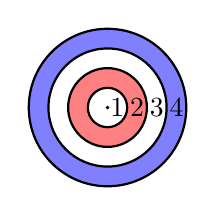
\begin{tikzpicture}[scale=0.25]
        % Outer circle (radius 4)
        \fill[blue!50] (0,0) circle (4);
        
        % Annular regions
        \fill[white] (0,0) circle (3);
        \fill[red!50] (0,0) circle (2);
        \fill[white] (0,0) circle (1);
        
        % Inner circle
        \fill[black] (0,0) circle (0.1); % A small black dot at the center
        
        % Draw the circle outlines
        \draw[thick] (0,0) circle (4);
        \draw[thick] (0,0) circle (3);
        \draw[thick] (0,0) circle (2);
        \draw[thick] (0,0) circle (1);
        
        % Labels
        \node at (3.5,0) {4}; % outermost region
        \node at (2.5,0) {3}; 
        \node at (1.5,0) {2}; 
        \node at (0.5,0) {1}; 
        
        
    \end{tikzpicture}
    \end{center}
 
\end{minipage}

\end{frame}



\begin{frame}{Solution to group exercise \#1}
\textbf{Problem.} Let $(S,P)$ be the probability space in which $S=\set{1,2,3,4}$. Suppose $P(1) =x, P(2) = 2x, P(3) = 3x,$ and  $P(4)=4x$.  Find $x$.
\vfill 
\textbf{Solution.} 

\begin{align*}
\sum_{s \in S} P(s) &= 1 && \scripttext{(Def. probability space)} \\
\implies P(1) + P(2) + P(3) + P(4) &=1	 && \scripttext{(Expand sum)} \\
\implies x + 2x + 3x + 4x &=1	 && \scripttext{(By assumption)} \\
\implies 10x &=1	 \\
\implies x &= \frac{1}{10}
\end{align*}

\vfill 
\textbf{Remark.} 

Therefore,
\[ P(1) = \frac{1}{10}, \quad  P(2) = \frac{2}{10}, \quad  P(3) = \frac{3}{10}, \quad  P(4) = \frac{4}{10}.\]



\end{frame}


\begin{frame}{Solution to group exercise \#2}
\textbf{Problem.}  Suppose that that $(S,P_1)$  and $(S,P_2)$ are two probability spaces that have the same set of outcomes, $S$.   Is it possible that each outcome is less likely in the first probability space than it is in the second?  That is, can we have $\forall s \in S, P_1(s) < P_2(s)$?
\vfill 
\textbf{Solution.}
No. By definition of a (finite) probability space, we have
%
\begin{align}
\sum_{s \in S} P_1(s) = \sum_{s \in S} P_2(s) = 1 
\label{eqn:prob_space_sums_to_one} 
\end{align}
%
But since $P_1(s) < P_2(s)$ for all $s$, we have
 %
\begin{align}
\sum_{s \in S} P_1(s) < \sum_{s \in S} P_2(s) 
\label{eqn:P2_dominates_P1} 
\end{align}
 %
Substituting \Eqref{eqn:prob_space_sums_to_one}  into \Eqref{eqn:P2_dominates_P1} , we obtain
\[ 1 < 1 \]
which is a contradiction.

   
\end{frame}


\begin{frame}{Remark on group exercise \#2}
\footnotesize  
\begin{figure}
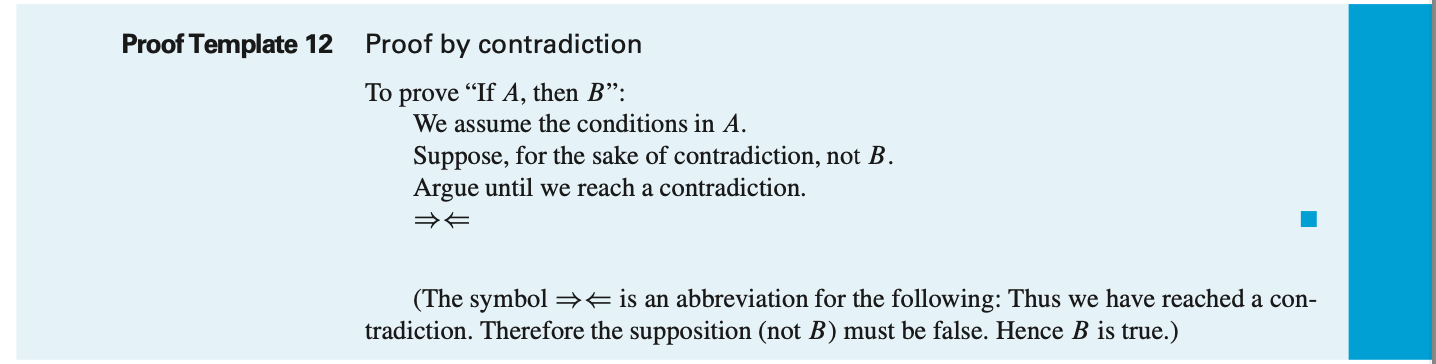
\includegraphics[width=\textwidth]{images/proof_by_contradiction.png}
\caption{\textit{A template for proof by contradiction.} Source: Scheinerman Sec. 20 (pp. 121)}	
\end{figure}
%
\vfill 
\begin{myredbox}[title=Remark]
 This is an example of proof by contradiction (Scheinerman Sec. 20).

% The solution to group exercise \#2 is an example of Proof by Contradiction.    

\begin{table}
\centering 	
\begin{tabularx}{\textwidth}{XX}
Proposition A: 	& $(S,P_1)$  and $(S,P_2)$ are two probability spaces that have the same set of outcomes, $S$.  \\
Proposition B: & $\forall s \in S, P_1(s) < P_2(s)$
\end{tabularx}
\end{table}

 We prove $A \implies (\texttt{not} \; B)$ by assuming $A$ and $B$ and obtaining a contradiction.	
\end{myredbox}
\end{frame}



\begin{frame}{Solution to group exercise \#3}
\footnotesize  
The areas of the circles are given by
%
\begin{align*}
C_1 &= \pi 1^2 = \pi   &  C_3 &= \pi 3^2 = 9 \pi  \\
C_2 &= \pi 2^2 = 4 \pi   &  C_4 &= \pi 4^2 = 16 \pi  
\end{align*}
%
Hence, the areas of the annular regions are given by 
%
\begin{align*}
A_1 &= C_1 = \pi  & A_3 &= C_3 - C_2 = 5 \pi  \\
A_2 &= C_2 - C_1 = 3 \pi  & A_4 &= C_4 - C_3 = 7 \pi  
\end{align*}
%
By assumption, the probability of the dart landing in each annular region is
\[ P(1) \propto A_1, \quad P(2) \propto A_2, \quad P(3) \propto A_3, \quad P(4) \propto A_4,\] 
where $\propto$ means \enquote{is proportional to}.  In other words,
\[ P(1) = \frac{A_1}{Z}, \quad P(2) = \frac{A_2}{Z}, \quad P(3) = \frac{A_3}{Z}, \quad P(4) = \frac{A_4}{Z},\]
where $Z$ is some unknown \enquote{normalizing constant}.  We solve for $Z$ by using that the probabilities over all outcomes must sum to unity: 
%
\begin{align*}
\sum_{s \in S} P(s) = 1  \implies \frac{A_1}{Z} + \frac{A_2}{Z} + \frac{A_3}{Z} + \frac{A_4}{Z}  = 1 \\
\implies A_1 + A_2 + A_3 + A_4 = Z  \implies Z = 16 \pi. 
\end{align*} 
%
Hence
\[ P(1) = \frac{1}{16}, \quad P(2) = \frac{3}{16}, \quad P(3) = \frac{5}{16}, \quad P(4) = \frac{7}{16}.\]
\end{frame}


\end{document}
